\documentclass{ximera}



\begin{document}



\subsection*{Catalog Description:}
Fractions and decimals, basic algebra, graphing lines, factoring, systems of equations. Credit for this course will not count toward graduation in any degree program.

\subsection*{Prerequisite:}
Math Placement Level T; or Math 1040 or 40 or 50; or permission of department.

\subsection*{Exclusions:}
Not open to students with credit for any Math course above 1050 (050).

\subsection*{Purpose of Course:}
Mathematics 1050 is designed to meet the needs of the students entering The Ohio State University at the lowest placement, course code T. This course will prepare students for Math 1075.

\subsection*{Follow-up Course:}
Math 1075

\subsection*{Sequencing Chart:}
\begin{image}
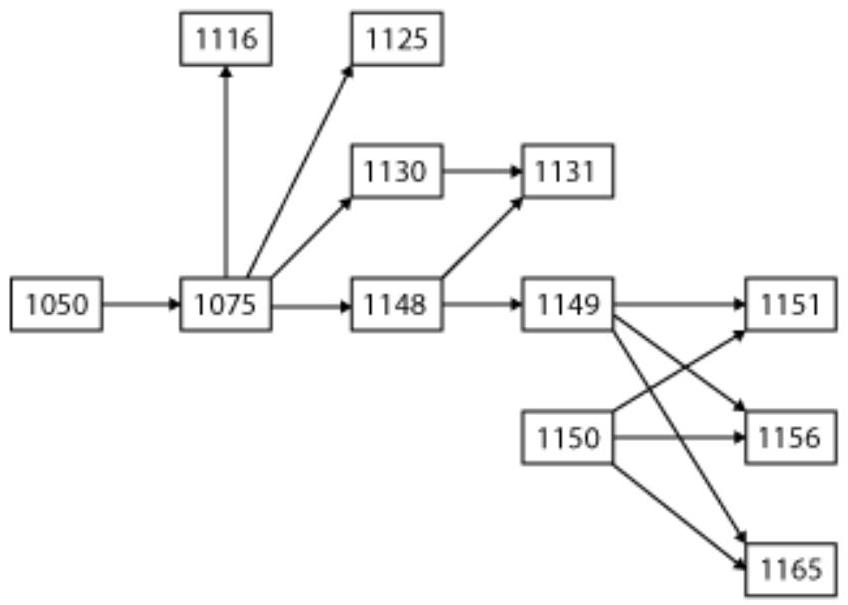
\includegraphics[alt={Flowchart showing Math course sequencing from 1050 through 1075 to upper-level courses including 1116, 1125, 1130, 1148, 1149, 1150, 1151, 1156, and 1165},width=\textwidth]{course-sequencing-chart.jpg}
\end{image}

\subsection*{Text:}
Beginning Algebra, $8{ }^{\text {th }}$ edition, by Aufmann \& Lockwood, Cengage, ISBN: 9781305942653\\
Topics List:\\
\begin{enumerate}
    \item
    \begin{enumerate}
        \item Section 1.1: Introduction to Integers
        \item Section 1.2: Operations with Integers
        \item Section 1.3: Rational Numbers
        \item Application 1: Addition of Fractions using Least Common Denominator
        \item Section 1.4 Exponents and the Order of Operations
        \item Section 1.5 Concepts from Geometry
    \end{enumerate}
    \item 
    \begin{enumerate}
        \item Section 2.1: Evaluating Variable Expressions
        \item Section 2.2: Simplifying Variable Expressions
        \item Section 2.3: Translating Verbal Expressions into Variable Expressions
    \end{enumerate}
    \item 
    \begin{enumerate}
        \item Section 3.1: Introduction to Equations
        \item Section 3.2: Applications of Equations of the Form $a x=b$
        \item Section 3.3: General Equations
        \item Section 3.4: Inequalities
    \end{enumerate}
    \item
    \begin{enumerate}
        \item Midterm 1
    \end{enumerate}  
    \item
    \begin{enumerate}
        \item Section 4.1: Translating Sentences into Equations
        \item Application 2: Integer, Coins, and Stamps Problems
        \item Section 4.2: Geometry Problems
        \item Section 4.3: Markup and Discount Problems
        \item Section 4.4: Investment Problems
        \item Section 4.5: Mixture Problems
        \item Section 4.6: Uniform Motion Problems
        \item Section 4.7: Inequalities
    \end{enumerate}
    \item
    \begin{enumerate}
        \item Section 5.1: The Rectangular Coordinate System
        \item Section 5.2: Graphs of Straight Lines
    \end{enumerate}
    \item
    \begin{enumerate}
        \item Midterm 2
    \end{enumerate}
    \item
    \begin{enumerate}
        \item Section 5.3: Slopes of Straight Lines
        \item Section 5.4: Equations of Straight Lines
        \item Section 5.6: Graphing Linear Inequalities
    \end{enumerate}
    \item 
    \begin{enumerate}
        \item Section 6.1: Solving Systems of Linear Equations by Graphing
        \item Section 6.2: Solving Systems of Linear Equations by the Substitution Method
        \item Section 6.3: Solving Systems of Linear Equations by the Addition Method
        \item Section 6.4: Application Problems in Two Variables
    \end{enumerate}
    \item 
    \begin{enumerate}
        \item Section 7.1: Addition and Subtraction of Polynomials
        \item Section 7.2: Multiplication of Monomials
        \item Section 7.3: Multiplication of Polynomials
        \item Section 7.4: Integer Exponents and Scientific Notation
        \item Section 7.5: Division of Polynomials
    \end{enumerate}
    \item 
    \begin{enumerate}
        \item Midterm 3
    \end{enumerate}
    \item 
    \begin{enumerate}
        \item Section 8.1: Common Factors
        \item Section 8.2: Factoring Polynomials of the Form $x^{2}+b x+c$
        \item Section 8.3: Factoring Polynomials of the Form $a x^{2}+b x+c$
        \item Section 8.4: Special Factoring
        \item Section 8.5: Factoring Polynomials Completely
        \item Section 8.6: Solving Equations
        \item Final
    \end{enumerate}
\end{enumerate}
\end{document}